%\documentclass[dvipdfmx]{beamer}      % platex の場合
\documentclass{beamer}                 % lualatex の場合
\usepackage{mySld}
\usepackage{multicol}

\begin{document}
\title{基礎コンピュータ工学\\第5章 機械語プログラミング\\(パート5)}
\date{}

\begin{frame}
  \titlepage
  \centerline{\url{https://github.com/tctsigemura/TecTextBook}}
  \vfill
  \centerline{本スライドの入手:
    \raisebox{-7mm}{
\includegraphics[scale=0.3]{../Img/QRs5_5.png}}}
\end{frame}

%==============================================================================
%\begin{frame}
%  \frametitle
%  \tableofcontents
%\end{frame}

\section{条件ジャンプ命令}
%==============================================================================
\begin{frame}
  \frametitle{フラグ(1)}
  フラグ(C,S,Z)は\emph{計算結果の特徴}を表す.\\
  フラグ変化ありの命令を実行する度に値が変化する.\\
  (教科書の本文,命令表を再度確認する.)
  \vfill
  \begin{itemize}
  \item \emph{Z(Zero)フラグ} \\
    \begin{itemize}
    \item Zero は「ゼロ」の意味.
    \vfill
    \item 計算の結果が\emph{ゼロ}にならなかった.
    {\small\begin{center}
      \begin{tabular}{ c r  c c r l}
                 & $0011~0010_2$ &    &   & $50_{10}$ & \\
        +        & $0011~0010_2$ & →  & + & $50_{10}$ & \\
        \cline{1-2} \cline{4-5}
        Z \fbox{0} & $0110~0100_2$ & ~ &  & $100_{10}$ &
      \end{tabular}
    \end{center}}
    \vfill
    \item 計算の結果が\emph{ゼロ}になった.
    {\small\begin{center}
      \begin{tabular}{ c r  c c r l}
                   & $0011~0010_2$ &    &            & $50_{10}$ & \\
        \texttt{-} & $0011~0010_2$ & →  & \texttt{-} & $50_{10}$ & \\
        \cline{1-2} \cline{4-5}
        Z \fbox{1} & $0000~0000_2$ & ~  &            & $0_{10}$ &
      \end{tabular}
    \end{center}}
    \end{itemize}
    \vfill
  \end{itemize}
  \vfill
\end{frame}

%==============================================================================
\begin{frame}
  \frametitle{フラグ(2)}
  \begin{itemize}
  \item \emph{S(Sign)フラグ} \\
    \begin{itemize}
    \item Sign はプラス・マイナスの「符号」の意味
    \vfill
    \item 計算の結果を符号付き2進数と解釈すると\emph{正の値}になった.
    {\small\begin{center}
      \begin{tabular}{ c r  c c r l}
                 & $0011~0010_2$ &    &   & $50_{10}$ & \\
        +        & $0011~0011_2$ & →  & + & $51_{10}$ & \\
        \cline{1-2} \cline{4-5}
        S \fbox{0} & $0110~0101_2$ & ~ &  & $101_{10}$ &
      \end{tabular}
    \end{center}}
    \vfill
    \item 計算の結果を符号付き2進数と解釈すると\emph{負の値}になった.
    {\small\begin{center}
      \begin{tabular}{ c r  c c r l}
                   & $0011~0010_2$ &    &            & $50_{10}$ & \\
        \texttt{-} & $0011~0011_2$ & →  & \texttt{-} & $51_{10}$ & \\
        \cline{1-2} \cline{4-5}
        S \fbox{1} & $1111~1111_2$ & ~  &            & $-1_{10}$ &
      \end{tabular}
    \end{center}}
    \end{itemize}
    \vfill
    \item \emph{Sフラグは符号付き2進数と考えたときの「負」の意味}
    \item 計算結果の最上位ビットと同じ値になる.→ゼロは「正」とみなす.
  \end{itemize}
  \vfill
\end{frame}

%==============================================================================
\begin{frame}
  \frametitle{フラグ(3)}
  \begin{itemize}
  \item \emph{C(Carry)フラグ} 
    \begin{itemize}
    \item Caryy は「桁を繰り上げる」の意味
    \vfill
    \item 足し算(ADD)で桁上げが起きる.
    \vfill
    \begin{itemize}
    \item 足し算で最上位桁からの桁上げがない場合 \\
    {\small\begin{center}
      \begin{tabular}{ c r  c c r l}
                 & $0111~1111_2$ &    &   & $127_{10}$ & \\
        +        & $0000~0001_2$ & →  & + &   $1_{10}$ & \\
        \cline{1-2} \cline{4-5}
        C \fbox{0} & $1000~0000_2$ & ~ &  &   $128_{10}$ & 
      \end{tabular}
    \end{center}}
    \vfill
    \item 足し算で最上位桁からの桁上げがあった場合(オーバーフロー) \\
    {\small\begin{center}
      \begin{tabular}{ c r  c c r l}
                 & $1111~1111_2$ &    &   & $255_{10}$ & \\
        +        & $0000~0001_2$ & →  & + &   $1_{10}$ & \\
        \cline{1-2} \cline{4-5}
        C \fbox{1} & $0000~0000_2$ & ~ &  &   $0_{10}$ & ?
      \end{tabular}
    \end{center}}
    \end{itemize}
    \vfill
    \end{itemize}
  \end{itemize}
  \vfill
\end{frame}

%==============================================================================
\begin{frame}
  \frametitle{フラグ(4)}
  \vfill
  \begin{itemize}
  \item \emph{C(Carry)フラグ}(Borrowの意味を\emph{代用})
    \begin{itemize}
    \item Borrow は「桁を借りる」の意味
    \vfill
    \item 引き算(SUB)で桁借りが起こる
    \vfill
    \begin{itemize}
    \item 引き算で最上位桁で桁借りがない場合
    \vfill
    {\small\begin{center}
      \begin{tabular}{ c r  c c r l}
                   & $1111~1111_2$ &    &            & $255_{10}$ & \\
        \texttt{-} & $0000~0001_2$ & →  & \texttt{-} &   $1_{10}$ & \\
        \cline{1-2} \cline{4-5}
        C \fbox{0} & $1111~1110_2$ & ~  &            & $254_{10}$ & ?
      \end{tabular}
    \end{center}}
    \vfill
    \item 引き算で最上位桁で桁借りがあった場合(負にオーバーフロー) 
    \vfill
    {\small\begin{center}
      \begin{tabular}{ c r  c c r l}
                   & $0000~0000_2$ &    &            & $0_{10}$ & \\
        \texttt{-} & $0000~0001_2$ & →  & \texttt{-} & $1_{10}$ & \\
        \cline{1-2} \cline{4-5}
        C \fbox{1} & $1111~1111_2$ & ~  &            & $255_{10}$ & ?
      \end{tabular}
    \end{center}}
    \end{itemize}
    \end{itemize}
    \vfill
    \item \emph{Cフラグは,符号なし2進数と考えたときのオーバーフローの意味}
  \end{itemize}
  \vfill
\end{frame}

%==============================================================================
\begin{frame}
  \frametitle{ジャンプ命令(7種類)}
  \begin{description}
  \item[無条件ジャンプ命令:]\emph{プログラムの流れ}を指定のアドレスに飛ばす.
    \begin{itemize}
      \item \emph{JMP(Jump)命令}:いつもジャンプする.
    \end{itemize}
    \vfill
  \item[条件ジャンプ命令:]ある条件のときだけジャンプする.
    \begin{itemize}
      \item \emph{JZ(Jump on Zero)命令}:$Z=1$ ならジャンプ
        \vfill
      \item \emph{JC(Jump on Carry)命令}:$C=1$ ならジャンプ
        \vfill
      \item \emph{JM(Jump on Minus)命令}:$S=1$ ならジャンプ
        \vfill
      \item \emph{JNZ(Jump on Not Zero)命令}:$Z=0$ ならジャンプ
        \vfill
      \item \emph{JNC(Jump on Not Carry)命令}:$C=0$ ならジャンプ
        \vfill
      \item \emph{JNM(Jump on Not Minus)命令}:$S=0$ ならジャンプ
    \end{itemize}
  \end{description}
  \vfill
\end{frame}

%==============================================================================
\begin{frame}
  \frametitle{JZ(Jump on Zero)命令}
  Zフラグが1なら(計算結果が0なら)ジャンプする.
  \vfill
  \begin{description}
  \item[フラグ:] 変化しない.
    \vfill

  \item[ニーモニック:]\texttt{JZ EA}~~~~~~~~~\texttt{(if(Z=1) PC ← EA)}
    \vfill

  \item[命令フォーマット:] 2バイトの長さを持つ.\\
    \twoByte{$1010_2$}{$01_2$~\XR}{\A}
    \vfill

  \item[フローチャート:] ある程度,自由にアレンジしてよい.\\
    \centerline{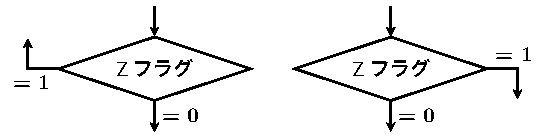
\includegraphics[scale=0.7]{../Tikz/jz.pdf}}
  \end{description}
  \vfill
\end{frame}

%==============================================================================
\begin{frame}
  \frametitle{JZ命令の使用例}
  ループを3回,繰り返すプログラム\\
  \vfill
  \begin{minipage}{0.4\columnwidth}
    \centerline{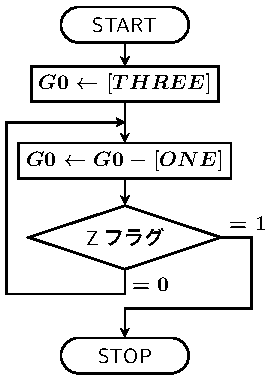
\includegraphics[scale=0.7]{../Tikz/flow0B.pdf}}
  \end{minipage}
  \begin{minipage}{0.59\columnwidth}
    {\ttfamily\small\begin{center}
      \begin{tabular}{|l|l|l|l l|} \hline
        番地 & 機械語 & ラベル & \multicolumn{2}{|c|}{ニーモニック} \\
        \hline
        00 & 10 09 &           & LD   & G0,THREE              \\
        02 & 40 0A &  LOOP     & SUB  & G0,ONE                \\
        04 & A4 08 &           & JZ   & STOP                  \\
        06 & A0 02 &           & JMP  & LOOP                  \\
        08 & FF    &  STOP     & HALT &                       \\
        09 & 03    &  THREE    & DC   & 3                     \\
        0A & 01    &  ONE      & DC   & 1                     \\
        \hline
      \end{tabular}
    \end{center}}
  \end{minipage}
  \vfill
  \begin{itemize}
  \item 演習(1):ステップモードで実行をトレースしてみる.
  \end{itemize}
\end{frame}

%==============================================================================
\begin{frame}
  \frametitle{JC(Jump on Carry)命令}
  Cフラグが1なら(オーバーフローなら)ジャンプする.
  \vfill
  \begin{description}
  \item[フラグ:] 変化しない.
    \vfill

  \item[ニーモニック:]\texttt{JC EA}~~~~~~~~~\texttt{(if(C=1) PC ← EA)}
    \vfill

  \item[命令フォーマット:] 2バイトの長さを持つ.\\
    \twoByte{$1010_2$}{$10_2$~\XR}{\A}
    \vfill

  \item[フローチャート:] ある程度,自由にアレンジしてよい.\\
    \centerline{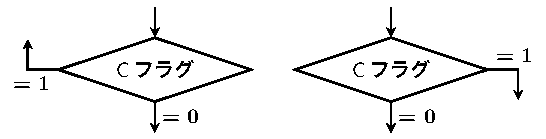
\includegraphics[scale=0.7]{../Tikz/jc.pdf}}
  \end{description}
  \vfill
\end{frame}

%==============================================================================
\begin{frame}
  \frametitle{JM(Jump on Minus)命令}
  Sフラグが1なら(負なら)ジャンプする.
  \vfill
  \begin{description}
  \item[フラグ:] 変化しない.
    \vfill

  \item[ニーモニック:]\texttt{JM EA}~~~~~~~~~\texttt{(if(S=1) PC ← EA)}
    \vfill

  \item[命令フォーマット:] 2バイトの長さを持つ.\\
    \twoByte{$1010_2$}{$11_2$~\XR}{\A}
    \vfill

  \item[フローチャート:] ある程度,自由にアレンジしてよい.\\
    \centerline{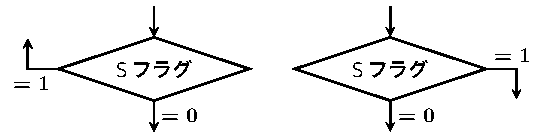
\includegraphics[scale=0.7]{../Tikz/jm.pdf}}
  \end{description}
  \vfill
\end{frame}

%==============================================================================
\begin{frame}
  \frametitle{条件判断1}
  計算結果により処理をするかしないか変化する例
  \vfill
  \begin{minipage}{0.49\columnwidth}
    \begin{itembox}[l]{\footnotesize 計算結果がゼロなら「処理」\emph{しない}}
      \centerline{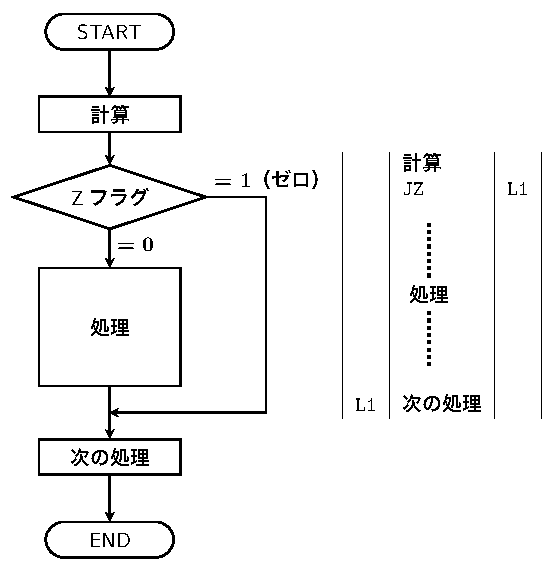
\includegraphics[scale=0.6]{../Tikz/flow2AB.pdf}}
    \end{itembox}
  \end{minipage}
  \begin{minipage}{0.5\columnwidth}
    \begin{itembox}[l]{\footnotesize 計算結果がゼロなら「処理」\emph{する}}
      \centerline{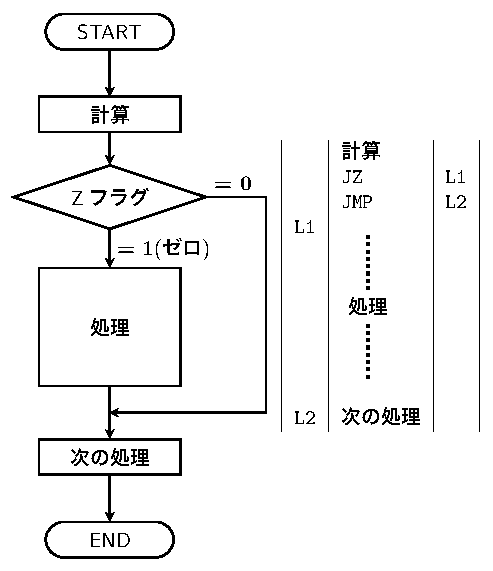
\includegraphics[scale=0.6]{../Tikz/flow2A.pdf}}
    \end{itembox}
  \end{minipage}
  \vfill
\end{frame}

%==============================================================================
\begin{frame}
  \frametitle{条件判断2}
  計算結果により\emph{どちらか}の処理をする例
  \vfill
  \begin{itembox}[l]{\footnotesize 計算結果がゼロなら「処理1」,
      そうでなければ「処理2」をする}
    \centerline{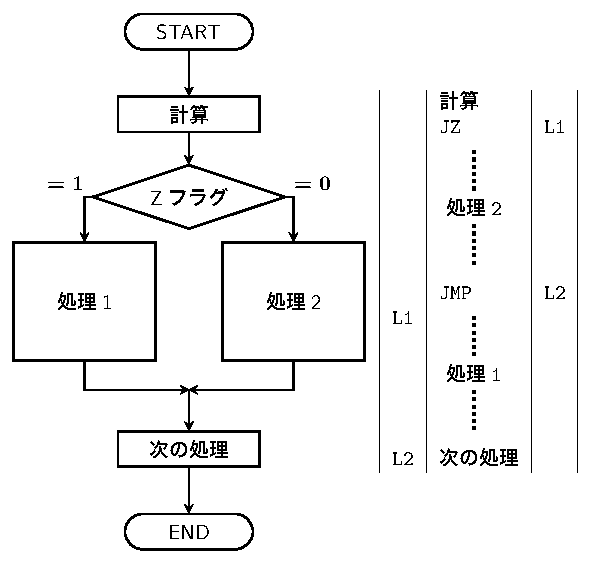
\includegraphics[scale=0.65]{../Tikz/flow2B.pdf}}
  \end{itembox}
  \vfill
\end{frame}

%==============================================================================
\begin{frame}
  \frametitle{条件判断の例}
  絶対値を求めるプログラム(例題5-1)\\
  \vfill
  \begin{minipage}{0.49\columnwidth}
    \centerline{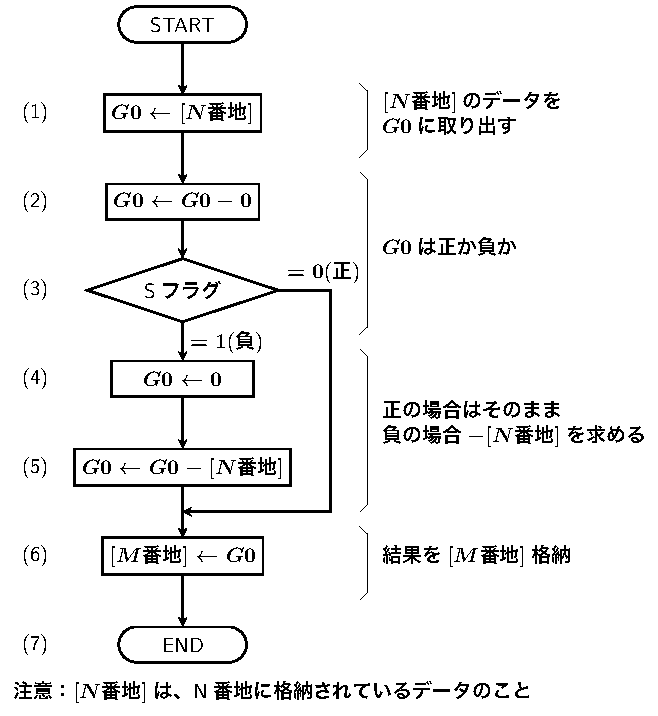
\includegraphics[scale=0.5]{../Tikz/flow1.pdf}}
  \end{minipage}
  \begin{minipage}{0.5\columnwidth}
    {\ttfamily\scriptsize\begin{center}
      \begin{tabular}{|l|l|l|l l|}
        \hline
        番地 & 機械語 & ラベル & \multicolumn{2}{|c|}{ニーモニック} \\
        \hline
        00 & 10 10 & START& LD   & G0,N    \\
        02 & 40 0F &      & SUB  & G0,ZERO \\
        04 & AC 08 &      & JM   & L1      \\
        06 & A0 0C &      & JMP  & L2      \\
        08 & 10 0F & L1   & LD   & G0,ZERO \\
        0A & 40 10 &      & SUB  & G0,N    \\
        0C & 20 11 & L2   & ST   & G0,M    \\
        0E & FF    &      & HALT &         \\
        0F & 00    & ZERO & DC   & 0       \\
        10 & FF    & N    & DC   & -1      \\
        11 & 00    & M    & DS   & 1       \\
        \hline
      \end{tabular}
    \end{center}}
  \end{minipage}
  \vfill
  \begin{itemize}
  \item 演習(2):ステップモードで実行をトレースしてみる.
  \end{itemize}
\end{frame}

%==============================================================================
\begin{frame}
  \frametitle{まとめ}
  \emph{学んだこと}
  \begin{itemize}
  \item フラグ(Carry,Zero,Sign)
  \item 条件ジャンプ命令(JZ,JC,JM)
  \item 条件判断
  \end{itemize}
  \vfill

  \emph{演習(宿題)}
  \begin{itemize}
  \item \emph{飽和演算}:計算結果が最大値または最小値を超えそうになった時,
    計算結果を最大値または最小値に留める演算方式
  \item TeCの符号なし2進数を用いて表現できる最大値は255である.
  \item 足し算結果が255を超える(オーバーフローする)かもしれない.
  \item オーバーフローが発生したら計算結果を255に訂正するようにする.
  \item 以上のような足し算プログラムを作る.
  \end{itemize}
  \vfill
\end{frame}

\end{document}
